\documentclass[11pt]{article}
\usepackage[T1]{fontenc}
\usepackage{lmodern}
\usepackage[margin=1.02in]{geometry}
\usepackage{microtype}
\usepackage{amsmath,amssymb,amsthm,mathtools,bm}
\usepackage{graphicx,xcolor,enumitem}
\usepackage{tikz}
\usetikzlibrary{calc,arrows.meta,positioning,fit,decorations.pathreplacing}
\usepackage[numbers,sort&compress]{natbib}
\usepackage[colorlinks=true,linkcolor=blue!45!black,citecolor=blue!45!black,urlcolor=blue!45!black]{hyperref}
\input{glyphtounicode}
\pdfglyphtounicode{angbracketleftBigg}{27E8}
\pdfglyphtounicode{angbracketleftbig}{27E8}
\pdfglyphtounicode{angbracketrightBigg}{27E9}
\pdfglyphtounicode{angbracketrightbig}{27E9}
\pdfglyphtounicode{arrowhookleft}{02D3}
\pdfglyphtounicode{axisshort}{002D}
\pdfglyphtounicode{arrowaxisright}{2192}
\pdfglyphtounicode{circleplusdisplay}{2A01}
\pdfglyphtounicode{circleplustext}{2A01}
\pdfglyphtounicode{braceex}{23AA}
\pdfglyphtounicode{braceleftbigg}{007B}
\pdfglyphtounicode{braceleftbt}{23A9}
\pdfglyphtounicode{braceleftmid}{23A8}
\pdfglyphtounicode{bracelefttp}{23A7}
\pdfglyphtounicode{bracerightbigg}{007D}
\pdfglyphtounicode{bracketleftbig}{005B}
\pdfglyphtounicode{bracketleftbigg}{005B}
\pdfglyphtounicode{bracketleftbt}{23A3}
\pdfglyphtounicode{bracketlefttp}{23A1}
\pdfglyphtounicode{bracketrightbig}{005D}
\pdfglyphtounicode{bracketrightbigg}{005D}
\pdfglyphtounicode{bracketrightbt}{23A6}
\pdfglyphtounicode{bracketrighttp}{23A4}
\pdfglyphtounicode{hatwide}{0302}
\pdfglyphtounicode{hatwider}{0302}
\pdfglyphtounicode{hatwidest}{0302}
\pdfglyphtounicode{integraldisplay}{222B}
\pdfglyphtounicode{integraltext}{222B}
\pdfglyphtounicode{intersectiondisplay}{22C2}
\pdfglyphtounicode{intersectiontext}{22C2}
\pdfglyphtounicode{mapsto}{007C}
\pdfglyphtounicode{parenleftBig}{0028}
\pdfglyphtounicode{parenleftBigg}{0028}
\pdfglyphtounicode{parenleftbig}{0028}
\pdfglyphtounicode{parenleftbigg}{0028}
\pdfglyphtounicode{parenleftbt}{239D}
\pdfglyphtounicode{parenlefttp}{239B}
\pdfglyphtounicode{parenrightBig}{0029}
\pdfglyphtounicode{parenrightBigg}{0029}
\pdfglyphtounicode{parenrightbig}{0029}
\pdfglyphtounicode{parenrightbigg}{0029}
\pdfglyphtounicode{parenrightbt}{23A0}
\pdfglyphtounicode{parenrighttp}{239E}
\pdfglyphtounicode{productdisplay}{220F}
\pdfglyphtounicode{producttext}{220F}
\pdfglyphtounicode{radicalbig}{221A}
\pdfglyphtounicode{radicalbigg}{221A}
\pdfglyphtounicode{radicalBigg}{221A}
\pdfglyphtounicode{floorleftbigg}{230A}
\pdfglyphtounicode{floorrightbigg}{230B}
\pdfglyphtounicode{ceilingleftBig}{2308}
\pdfglyphtounicode{ceilingrightBig}{2309}
\pdfglyphtounicode{summationdisplay}{2211}
\pdfglyphtounicode{summationtext}{2211}
\pdfglyphtounicode{uniontext}{22C3}
\pdfglyphtounicode{vextenddouble}{2225}
\pdfglyphtounicode{vextendsingle}{007C}
\pdfglyphtounicode{tildewide}{0303}
\pdfglyphtounicode{tildewider}{0303}
\pdfglyphtounicode{bracketleftBigg}{005B}
\pdfglyphtounicode{bracketrightBigg}{005D}
\pdfglyphtounicode{braceleftBigg}{007B}
\pdfglyphtounicode{bracerightBigg}{007D}
\pdfglyphtounicode{braceleftBig}{007B}
\pdfglyphtounicode{bracerightBig}{007D}
\pdfglyphtounicode{coproductdisplay}{2210}
\pdfglyphtounicode{bracketleftBig}{005B}
\pdfglyphtounicode{bracketrightBig}{005D}
\pdfglyphtounicode{radicalBig}{221A}
\pdfglyphtounicode{uniondisplay}{22C3}
\pdfglyphtounicode{logicalandtext}{22C0}
\pdfglyphtounicode{logicalanddisplay}{22C0}
\pdfglyphtounicode{circlemultiplytext}{2A02}
\pdfglyphtounicode{circlemultiplydisplay}{2A02}
\pdfglyphtounicode{braceleftbig}{007B}
\pdfglyphtounicode{bracerightbig}{007D}
\pdfglyphtounicode{bracerighttp}{23AB}
\pdfglyphtounicode{bracerightmid}{23AC}
\pdfglyphtounicode{bracerightbt}{23AD}
\pdfgentounicode=1


\hypersetup{pdftitle={Boundedness and persistence of weakly reversible mass-action systems},pdfauthor={OpenAI}}
\newcommand{\R}{\mathbb R}
\newcommand{\N}{\mathbb N}
\newcommand{\norm}[1]{\lVert#1\rVert}
\newcommand{\abs}[1]{\lvert#1\rvert}
\newcommand{\ip}[2]{\langle#1,#2\rangle}
\newtheorem{theorem}{Theorem}[section]
\newtheorem{lemma}[theorem]{Lemma}
\newtheorem{proposition}[theorem]{Proposition}
\newtheorem{corollary}[theorem]{Corollary}
\theoremstyle{definition}
\newtheorem{definition}[theorem]{Definition}
\theoremstyle{remark}
\newtheorem{remark}[theorem]{Remark}
\newtheorem{example}[theorem]{Example}
\numberwithin{equation}{section}
\title{Boundedness and persistence of\\weakly reversible mass-action systems}
\author{OpenAI}
\date{September 25, 2026}
\begin{document}
\maketitle
\begin{abstract}
We prove the boundedness and persistence conjectures for finite weakly
reversible mass-action systems with positive constant reaction rates.
For every positive initial condition, the solution exists for all forward
time, and every concentration remains bounded above and bounded away from
zero. The bounds may depend on the initial condition, and no boundedness
assumption is imposed on its stoichiometric compatibility class.
\end{abstract}
\section{Introduction}
\label{sec:introduction}

Weak reversibility is a condition on the directed graph of a chemical
reaction network: each reaction has a directed return path. Two central
questions ask whether this condition alone prevents species extinction
under mass-action kinetics and whether every positive trajectory remains
bounded. We prove the joint boundedness and persistence conclusion for
arbitrary positive constant reaction rates, any number of connected
components in the
reaction graph, and every species dimension.

\subsection{The problem and main result}

A finite reaction network with $d\ge1$ species consists of a finite set of
\emph{complexes} $\mathcal C\subset\mathbb Z_{\ge0}^d$ and a set
$\mathcal R\subset\{(y,y'):y,y'\in\mathcal C,\ y\ne y'\}$ of directed
reactions. We write a reaction as $y\to y'$. The network is
\emph{weakly reversible} if, for each $y\to y'\in\mathcal R$, there is a
directed path from $y'$ to $y$. A connected component of the underlying
undirected reaction graph is called a \emph{linkage class}. There is no
restriction on their number. Empty reaction sets and isolated complexes
are allowed.

Assign a positive constant $\kappa_{y\to y'}$ to each reaction. The
mass-action equation is
\begin{equation}\label{eq:mass-action}
 \dot x=f(x):=
 \sum_{y\to y'\in\mathcal R}
 \kappa_{y\to y'}x^y(y'-y),
 \qquad x^y:=\prod_{i=1}^d x_i^{y_i}.
\end{equation}
Since the exponents are nonnegative integers, $f$ is a polynomial vector
field. A forward trajectory in $\R_{>0}^d$ is called \emph{persistent} if
\[
 \liminf_{t\to\infty}x_i(t)>0\qquad(1\le i\le d).
\]
The bounds in this definition may depend on the trajectory.

\begin{theorem}\label{thm:main}
Let $d\ge1$, let $\mathcal C\subset\mathbb Z_{\ge0}^d$ be finite, let $\mathcal R$ be
weakly reversible, and let all reaction rates be positive constants.
For every $x^0\in\R_{>0}^d$, the solution of \eqref{eq:mass-action} with
$x(0)=x^0$ exists for every $t\ge0$. There is a number
$\varepsilon\in(0,1)$, depending on the network, the rates, and $x^0$, such
that
\begin{equation}\label{eq:main-bounds}
 \varepsilon\le x_i(t)\le\varepsilon^{-1}
 \qquad(t\ge0,\ 1\le i\le d).
\end{equation}
\end{theorem}

In particular, every positive trajectory is bounded and persistent.
To relate the statement to conservation laws, put
\[
 S=\operatorname{span}_{\R}\{y'-y:y\to y'\in\mathcal R\},
 \qquad
 P=(x^0+S)\cap\R_{\ge0}^d.
\]
The subspace $S$ is the \emph{stoichiometric subspace}, and $P$ is the
closed \emph{stoichiometric compatibility class} of $x^0$. Since $f(x)$
takes values in $S$, integration of the equation shows that a positive
trajectory starting at $x^0$ stays in $P$.
Theorem~\ref{thm:main} applies whether or not $P$ is bounded. It therefore
includes the persistence question for bounded entire compatibility
classes. The estimate \eqref{eq:main-bounds} also shows directly that the
omega-limit set is nonempty and disjoint from the orthant boundary:
every sequence of times tending to infinity has a subsequence along which
the trajectory converges inside the compact positive box in
\eqref{eq:main-bounds}.
We make no assertion in this generality that the trajectory converges to an
equilibrium, or that the same $\varepsilon$ works for all positive initial
points.
In particular, the theorem does not assert uniform eventual bounds over
all positive initial points in a compatibility class.

The proof gives a geometric strengthening, stated precisely in
Proposition~\ref{prop:polytope}: each $x^0>0$ belongs to a compact convex
polytope $K\subset\R_{>0}^d$ such that every solution starting in $K$
exists globally and remains in $K$. The set $K$ need not be a whole
compatibility class. It is constructed in the ambient species space and
may meet several such classes. Its convexity also yields a short proof
of the known existence theorem of Boros~\cite{Boros2019}: every positive
stoichiometric class contains a positive equilibrium
(Corollary~\ref{cor:positive-equilibrium}).

\subsection{History and the role of the construction}

The classical structural theory begins with complex balance.
A system is \emph{complex-balanced} if it admits a positive state at
which the total incoming and outgoing reaction fluxes agree at every
complex. Horn and Jackson's equilibrium and stability
theory~\cite{HornJackson1972}, Horn's complex-balancing
criteria~\cite{Horn1972}, and Feinberg's deficiency-zero
analysis~\cite{Feinberg1972} provide the foundations. Weak reversibility
is a property of the graph, whereas complex balance also depends on the
rates. The global-attractor question for complex-balanced systems asks
whether every positive trajectory converges to the unique positive
equilibrium in its stoichiometric class. This convergence follows from
Theorem~\ref{thm:main} under the additional complex-balance assumption;
Remark~\ref{rem:complex-balanced-convergence} gives the argument.

Feinberg~\cite[Remark~6.1.E]{Feinberg1987} formulated the weaker
expectation that a positive trajectory of a weakly reversible mass-action system
cannot converge to a point where a species concentration is zero.
Persistence excludes approach to the boundary along any sequence of
times. Anderson~\cite[Section~1.1]{Anderson2011} separated the
\emph{boundedness conjecture}, that positive trajectories of weakly
reversible mass-action systems are bounded, from the
\emph{persistence conjecture} for bounded trajectories. Together these
imply persistence without an assumed upper bound.
Theorem~\ref{thm:main} establishes both conclusions for arbitrary
positive constant reaction rates.

August and Barahona~\cite[Theorem~6]{AugustBarahona2010} previously stated
the general boundedness and persistence conclusion. Their proof, Part~III
on page~45 before Equation~(11), infers monomial dominance from a maximal
sum of exponents and a sufficiently large product of concentrations.
That implication does not hold throughout the stated region. In
$2A\rightleftarrows B$ with both rates one, the concentrations
$(a,b)=(T,T^3)$ satisfy $ab\to\infty$ but $a^2<b$, and
\[
 \dot a+\dot b=b-a^2=T^3-T^2>0\qquad(T>1).
\]
This contradicts the asserted implication. It does not contradict their
theorem: $a+2b$ is conserved in this example. Our proof controls the
relevant exponent pairings separately and establishes the conclusion
independently.

Several earlier results give classwise permanence or permit
time-dependent rates. Here \emph{permanence} means that, for each fixed
compatibility class, there is a compact subset of the positive orthant
that eventually contains every positive trajectory in that class, with
entry time depending on the initial state.
Anderson~\cite{Anderson2011} proved boundedness for weakly reversible
systems with a single linkage class. Gopalkrishnan, Miller, and
Shiu~\cite{GopalkrishnanMillerShiu2014} proved permanence for the larger
class of strongly endotactic systems, which includes every weakly
reversible single-linkage system; Boros and
Hofbauer~\cite{BorosHofbauer2020} gave a later proof of the single-linkage
result. Craciun, Nazarov, and Pantea~\cite{CraciunNazarovPantea2013}
proved boundedness, persistence, and permanence for two-species weakly
reversible systems as part of their more general endotactic result.
Pantea~\cite{Pantea2012} proved persistence of bounded weakly reversible
trajectories when the stoichiometric subspace has dimension two, with
arbitrary species and linkage counts. Two species and two-dimensional
stoichiometry are different restrictions. These results also permit
rates that vary in time while remaining bounded above and away from
zero. Our theorem treats constant rates in all dimensions and with any
number of linkage classes. Its bounds may depend on the initial point,
so it does not assert the classwise uniformity of permanence.

The revised toric-differential-inclusion approach of
Craciun~\cite[Section~8, final remark, p.~81]{Craciun2026}, in version~3
dated September~23, 2026, gives persistence for bounded positive
trajectories of weakly reversible systems with uniformly positive and
bounded variable rates. Its complex-balanced application combines the
boundary construction with the Horn--Jackson Lyapunov bound. The general
weakly reversible statement assumes a trajectory upper bound.
Our construction supplies that bound together with persistence, through
a compact convex forward-invariant polytope containing each prescribed
positive initial point.

The geometric and analytical methods also have substantial antecedents.
Invariant polygons and quantitative monomial comparisons appear in
Craciun, Nazarov, and Pantea~\cite{CraciunNazarovPantea2013}, and
projected polyhedra in Pantea~\cite{Pantea2012}. Anderson's monomial
tiers and return-path domination~\cite{Anderson2011Global}, the
projection and multiscale arguments of Gopalkrishnan, Miller, and
Shiu~\cite{GopalkrishnanMillerShiu2013,GopalkrishnanMillerShiu2014},
and Craciun's ordered-complex embedding into toric differential
inclusions~\cite{Craciun2019} organize related comparisons. Our
finite affine-label construction and directed-cut estimate are proved
directly; none of these research results is an input to the proof.

\subsection{Proof overview}

The obstacle is to find a single finite family of linear inequalities
that controls both small and large concentrations. An individual reaction
need not point inward across a proposed face. Weak reversibility supplies
return paths, so the inward estimate will concern the combined flux across
cuts of the reaction graph. The normal of each active face must make
strict comparisons that agree with the monomial sizes. Near a tie, an
arbitrary approximation to a normal can reverse a comparison; the geometric
construction must respect these ties.

For $0<h<1$ and $p\in[-1,1]^d$, write
\[
 X_h(p)=(h^{p_1},\ldots,h^{p_d}).
\]
These points fill the box $B_h=[h,h^{-1}]^d$. We construct a concave
piecewise-affine function
\[
 F_h(x)=\min_{\lambda\in\Lambda}
       \bigl(r_\lambda\cdot x+c_\lambda(h)\bigr),
\]
where $\Lambda$ is a finite set indexing the affine functions, and the
slopes $r_\lambda\in[-1,1]^d$ are independent of $h$. A label
$\lambda$ is \emph{active} at $x$ if its affine function attains this
minimum; every minimizer is active at a tie.

Lemma~\ref{lem:affine} and Corollary~\ref{cor:uniform-affine} supply the
family for any positive tolerance $E:[-1,1]^d\to(0,\infty)$:
for all sufficiently small $h$, every label active at $X_h(p)$ satisfies
$\norm{p-r_\lambda}_\infty<E(r_\lambda)$, uniformly over the cube.
No continuity of $E$ is required. We can therefore make the tolerance
small near the hyperplanes where a coordinate or a complex comparison
vanishes, while keeping it positive on those hyperplanes. This forces
each nonzero slope comparison to have the same sign as the corresponding
exponent comparison, with a fixed positive gap. In particular, for some
$H>0$ independent of $h$,
\[
 r_\lambda\cdot y<r_\lambda\cdot z
 \quad\Longrightarrow\quad x^z\le h^H x^y
 \qquad(x=X_h(p),\ \lambda\text{ active}).
\]
The parameter order is essential: first the tolerance, then the fixed
finite slopes, then their positive separation $H$, and only then the
final value of $h$. A finite covering by nearby slopes alone would not
ensure that the slopes attaining the minimum have the required accuracy.

Order the complexes by an active slope. Across a cut between two
successive distinct levels, weak reversibility supplies an upward reaction
whenever there is a downward reaction. The monomial comparison makes one
upward rate dominate the sum of all downward rates once $h$ is small
enough. Summing over the cuts gives $r_\lambda\cdot f(x)\ge0$ for
every active label. Consequently $F_h$ is nondecreasing along any
trajectory segment in $B_h$. At a tie, its right derivative is the
minimum of the derivatives of all active branches, so controlling a
preferred active label would not suffice. Equal slope levels need not
have equal monomials; edges within one level contribute zero to the
normal derivative.

The coordinate comparisons force every label active at the prescribed
$x^0$ to have slope zero when $h$ is sufficiently small. Fixing such a
label gives a constant branch with value $M=F_h(x^0)$ and hence the
global bound $F_h\le M$. The maximum set
\[
 K=\{x\in\R^d:F_h(x)=M\}
\]
is an intersection of finitely many closed affine half-spaces and
contains $x^0$. A zero slope cannot be active on $\partial B_h$, so
$K$ misses that boundary. Convexity now places all of $K$ inside $B_h$:
a segment from $x^0$ to any point outside the box would meet its boundary.
Thus $K$ is a compact positive polytope. Along a solution starting in
$K$, nondecrease of $F_h$ and the ceiling $M$ force the solution to
remain in the maximum set. A first-exit argument and compact continuation
prove invariance and global existence, giving the trajectory bounds.
No active-label estimate outside $B_h$ is needed.

Section~\ref{sec:affine} proves the approximation lemma by induction on
dimension and finite gluing over the minimum exponent, then obtains its
uniform form. Section~\ref{sec:dynamics} imposes the sign constraints,
proves the cut and derivative estimates, constructs the invariant polytope,
and deduces the trajectory bounds, positive-equilibrium existence and
complex-balanced convergence.

\section{Affine labels with a prescribed tolerance}
\label{sec:affine}

We construct a finite minimum of affine functions whose minimizing slopes
approximate the exponents of a positive point.  The permitted error is
prescribed separately at each slope.  Allowing this prescription to be
discontinuous will let us impose sign conditions on finitely many linear
forms in the application.

For an integer $m\geq 1$, $u\in\R^m$, and $0<h<1$, write
\[
  X_h(u)=(h^{u_1},\ldots,h^{u_m}).
\]
A \emph{label} is a pair $(r,c)$ consisting of a vector $r\in\R^m$,
independent of $h$, and a real-valued offset $c(h)$ defined for all
sufficiently small positive $h$.  For a finite nonempty family $\Lambda$
of labels, write its members as $\lambda=(r_\lambda,c_\lambda)$.
For fixed sufficiently small $h>0$ and $x\in\R^m$, a label
$\lambda\in\Lambda$ is \emph{active at $x$} if
\[
  r_\lambda\cdot x+c_\lambda(h)
  =\min_{\eta\in\Lambda}\bigl(r_\eta\cdot x+c_\eta(h)\bigr).
\]
Thus every minimizing label is active when a tie occurs.  Whenever finitely
many families are combined, we restrict their offsets to a common interval
$0<h<h_*$ on which they are all defined.

\begin{lemma}[Affine approximation with arbitrary tolerance]
\label{lem:affine}
Let $m\geq 1$ be an integer, let $a<b$ be real numbers, and let
$E:[a,b]^m\to(0,\infty)$ be any function.  There is a finite nonempty
family $\Lambda$ of labels $\lambda=(r_\lambda,c_\lambda)$, with
$r_\lambda\in[a,b]^m$ and $c_\lambda(h)=o(h^a)$ as $h\to0+$, such
that the following holds.
For every sequence $h_\nu\to0+$ and every sequence $p^\nu\in\R^m$
converging to $p\in[a,b]^m$, if a fixed label $\lambda\in\Lambda$ is
active at $X_{h_\nu}(p^\nu)$ for every $\nu$, then
\[
  \norm{p-r_\lambda}_\infty<E(r_\lambda).
\]
No regularity of $E$ is assumed, and the approximating vectors $p^\nu$
need not belong to $[a,b]^m$.
\end{lemma}

Two aspects of the statement will be used separately. The slopes form a
fixed finite set, rather than a set that changes with $h$. Also, the
conclusion concerns every label that stays active along a sequence,
including labels tied with other minimizers. The freedom for $p^\nu$ to
leave the cube is needed by the induction: a projected sequence may
approach a face of a smaller cube from either side.

\begin{proof}
We induct on $m$, using only positive dimensions smaller than $m$.
The largest coordinate of $X_h(p)$ is $h^{\min_i p_i}$, so we first
construct a family for each fixed value of the smallest exponent.
Within that family, negative offsets compensate for raising slope entries
on the smaller coordinates of $X_h(p)$.
Compactness extends the family's guarantee to nearby minimum
values, and a finite interval construction then selects among these
families. When $m=1$, the first step
uses singleton families and invokes no induction hypothesis; the remaining
steps therefore also establish the base case.

\medskip
\noindent\emph{Step 1: construction at a fixed minimum.}
Set $\mu(u)=\min_i u_i$, write $\mathbf 1=(1,\ldots,1)$, and fix
$t\in[a,b]$.  We will construct a finite
family $\Lambda_t$ whose slopes all satisfy $\mu(r)=t$, containing
$(t\mathbf 1,0)$, with the following property: the conclusion of the lemma
holds for activity within $\Lambda_t$ whenever the limiting vector
$p\in[a,b]^m$ satisfies $\mu(p)=t$.

If $m=1$ or $t=b$, take $\Lambda_t=\{(t\mathbf 1,0)\}$.  In either
case, a limit in the cube with minimum $t$ must equal $t\mathbf 1$, so
the asserted property holds.  Assume henceforth in this construction that
$m>1$ and $t<b$.

A label has \emph{type $k$} if precisely $k$ entries of its slope are
strictly greater than $t$, with all other entries equal to $t$.  Type $0$
consists of $(t\mathbf 1,0)$.  Construct types $k=1,\ldots,m-1$ in
increasing order.  After type $k-1$ has been constructed, choose $\beta_k$
so that
\begin{gather*}
  t<\beta_k<b,\qquad
  \beta_k<\beta_{k-1}\quad\text{if }k>1,\\
  \beta_k-t<E(r)
  \quad\text{for every slope $r$ of type $k-1$.}
\end{gather*}
The already constructed type has finitely many slopes, and its tolerance
values are all positive, so such a choice is possible. Only those finitely
many values are compared; we do not take a positive lower bound for $E$
on an entire cube.

For each $k$-element subset $U\subset\{1,\ldots,m\}$ and each
$s\in[\beta_k,b]^U$, let $r(s)\in[a,b]^m$ have entries $s$ on $U$ and
$t$ off $U$.  Apply the induction hypothesis in dimension $k$ to
$[\beta_k,b]^U$, with tolerance $s\mapsto E(r(s))$; the coordinates of
$U$ are taken in their natural order.  For every resulting label $(s,d)$,
where $d(h)=o(h^{\beta_k})$, put the label
\[
  r=r(s),\qquad c(h)=-h^{\beta_k}+d(h)
\]
in type $k$.  Taking all such coordinate sets and types gives a finite
nonempty family $\Lambda_t$.  Each of its offsets is $o(h^t)$.
The negative term $-h^{\beta_k}$ favors raising slope entries when
the corresponding coordinates of $x$ are small relative to $h^t$; the decreasing
$\beta_k$ make this preference stronger at each successive type.

\medskip
\noindent\emph{Step 2: verification at the fixed minimum.}
For the construction with $m>1$ and $t<b$, suppose $h_\nu\to0+$,
$p^\nu\to p\in[a,b]^m$, and $\mu(p)=t$.
Fix a label $(r,c)$ of type $k$ that is active within $\Lambda_t$ along this
sequence, and let $U$ be its set of raised coordinates.  All asymptotic
comparisons in this verification are along the sequence, and we write
$h=h_\nu$. Whenever a limiting exponent is strictly above or below a
threshold, convergence leaves a fixed positive exponent gap for all large
$\nu$. We use these gaps, not a replacement of $h^{p_i^\nu}$ by
$h^{p_i}$: convergence of the exponents alone would not justify that
replacement.

If $k>0$, comparison with $(t\mathbf 1,0)$ gives
\[
  \sum_{i\in U}(r_i-t)h^{p_i^\nu}
  \leq h^{\beta_k}-d(h)
  =(1+o(1))h^{\beta_k}.
\]
Every coefficient on the left is at least $\beta_k-t>0$.  If some
$p_i<\beta_k$ for $i\in U$, then, for a fixed $\delta>0$ and all
sufficiently large $\nu$, $p_i^\nu\leq\beta_k-\delta$; dividing the
display by $h^{\beta_k}$ would yield a term tending to infinity.
Consequently
\[
  p_i\geq\beta_k\quad(i\in U).
\]
Among labels constructed from this same $U$, the contributions off $U$
and the offset $-h^{\beta_k}$ are common.  Thus $(s,d)$ is active in the
family supplied by induction.  Its limiting exponent vector belongs to
$[\beta_k,b]^U$, so the induction hypothesis yields
\[
  \max_{i\in U}\abs{p_i-r_i}<E(r).
\]
This is precisely where unrestricted approximating vectors are needed:
$p_U^\nu$ may lie outside $[\beta_k,b]^U$ even though its limit lies
inside that cube. In particular, no strict inequality is required when a
limiting coordinate equals $\beta_k$ or $b$.

We next control the coordinates off $U$, including type $0$ by taking
$U=\varnothing$.  Suppose $k<m-1$.  We claim that
\[
  p_i\leq\beta_{k+1}\quad(i\notin U).
\]
If instead $p_j>\beta_{k+1}$ for some $j\notin U$, then every limiting
exponent on $U\cup\{j\}$ is strictly greater than $\beta_{k+1}$.
For $k>0$, this uses $p_i\geq\beta_k>\beta_{k+1}$ on $U$; for $k=0$
there are no such coordinates to check.  Choose any type $k+1$ label
whose raised set is $U\cup\{j\}$.  Its affine value minus the value of
$(t\mathbf 1,0)$ is
\[
  -h^{\beta_{k+1}}+o(h^{\beta_{k+1}}),
\]
because $h^{p_i^\nu}=o(h^{\beta_{k+1}})$ on every raised coordinate.
The corresponding difference for the supposed active label is zero if
$k=0$, and is bounded below by
$-h^{\beta_k}+o(h^{\beta_k})$ if $k>0$.
Since $h^{\beta_k}=o(h^{\beta_{k+1}})$ in the latter case, the chosen
competitor has a strictly smaller value for all sufficiently large $\nu$,
a contradiction.  This proves the claim.  Because $p_i\geq t$ and
$r_i=t$ off $U$, it follows that
\[
  \abs{p_i-r_i}\leq\beta_{k+1}-t<E(r)
  \quad(i\notin U),
\]
where the strict inequality was imposed when constructing type $k+1$.

If instead $k=m-1$, the sole coordinate off $U$ has limiting exponent
exactly $t$: all coordinates on $U$ have exponent at least
$\beta_k>t$, and $\mu(p)=t$.  Its error is therefore zero.  Combining
the bounds proves $\norm{p-r}_\infty<E(r)$ in all cases, including
types $0$ and $m-1$.  No strictness was required at a threshold
$p_i=\beta_k$.

\medskip
\noindent\emph{Step 3: extension to nearby minima.}
Keep $t$ and its finite family $\Lambda_t$ fixed.  For a label
$\lambda=(r,c)$ in that family, let $A_\lambda\subset[a,b]^m$ be the
set of all limits of sequences $p^\nu\in\R^m$ for which
$h_\nu\to0+$ and $\lambda$ is active within $\Lambda_t$ at
$X_{h_\nu}(p^\nu)$.
This set is closed.  Indeed, if $z_n\in A_\lambda$ and $z_n\to z$,
choose from a realizing sequence for $z_n$ a point $u_n$ and parameter
$h_n$ such that
\[
  0<h_n<1/n,\qquad \norm{u_n-z_n}_\infty<1/n,
\]
and $\lambda$ is active at $X_{h_n}(u_n)$.  Then $u_n\to z$, so
$z\in A_\lambda$. This diagonal selection uses actual active points;
it does not pass activity through a continuity assertion about $c(h)$.

The set
\[
  B_t=\bigcup_{\lambda=(r,c)\in\Lambda_t}
  \bigl\{p\in A_\lambda:\norm{p-r}_\infty\geq E(r)\bigr\}
\]
is therefore compact.  Here each $E(r)$ is a fixed real number;
continuity of $E$ is unnecessary.  The fixed-minimum verification shows
that $B_t$ contains no point with $\mu(p)=t$.  Since $\mu$ is continuous,
there is $\rho_t>0$ such that $B_t$ contains no point with
\[
  \mu(p)\in I_t:=(t-\rho_t,t+\rho_t).
\]
For example, if $B_t$ is nonempty, take $\rho_t$ smaller than the
positive minimum of $\abs{\mu(p)-t}$ on $B_t$; if it is empty, any
positive radius initially suffices.  Thus the limiting active-label
conclusion holds whenever $p\in[a,b]^m$ and $\mu(p)\in I_t$.

Shrink $\rho_t$, if necessary, so that every local offset also satisfies
\begin{equation}
  c(h)=o(h^{t+\rho_t}).
  \label{eq:affine-local-decay}
\end{equation}
For a nonsingleton family it suffices to require
$t+\rho_t<\min_{1\leq k\leq m-1}\beta_k$; for a singleton family the
offset is zero. The stronger decay uses the constructed form
$c(h)=-h^{\beta_k}+o(h^{\beta_k})$ with $\beta_k>t$; it would not follow
from $c(h)=o(h^t)$ alone. Shrinking the radius preserves the guarantee
just proved.
We have now obtained the desired approximation near every possible value
of $\mu(p)$.  It remains to make a finite combined family select an
appropriate one of these neighborhoods.

\medskip
\noindent\emph{Step 4: finite interval construction and combination.}
The local families already approximate correctly near their own minimum
levels. We now give each family a common offset shift so that a globally
active label must come from a suitable neighborhood. The overlap between
neighboring neighborhoods is important: it permits equality at the
transition cuts.

Choose a finite subcover of $[a,b]$ from the intervals $I_t$.  Remove
intervals contained in another selected interval, retaining one copy if
two coincide.  Order the remaining centers as
\mbox{$a\leq t_1<\cdots<t_N\leq b$}, and write
$I_{t_j}=(L_j,R_j)$.  Noncontainment forces the orders of the left and
right endpoints to agree; since $t_j=(L_j+R_j)/2$, both orders agree
with that of the centers.  Hence
\[
  L_1<\cdots<L_N,\qquad R_1<\cdots<R_N.
\]
Successive intervals overlap.  Otherwise $R_j\leq L_{j+1}$, and a
point of $[R_j,L_{j+1}]\subset(t_j,t_{j+1})$ would be covered by none
of the selected intervals.  The first interval contains $a$ and the
last contains $b$, by the endpoint orders, coverage, and the fact that
all centers lie in $[a,b]$.

For $1\leq j<N$, choose
\[
  q_j\in
  \bigl(\max\{t_j,L_{j+1}\},\,
        \min\{t_{j+1},R_j\}\bigr).
\]
This open interval is nonempty: the two intervals overlap, each contains
its own center, and $t_j<t_{j+1}$.  Thus $q_j$ belongs to both adjacent
intervals and lies strictly between their centers.  Setting $q_0=a$ and
$q_N=b$, we obtain
\begin{equation}
  t_j<q_j<t_{j+1}\quad(1\leq j<N),\qquad
  [q_{j-1},q_j]\subset I_{t_j}\quad(1\leq j\leq N).
  \label{eq:affine-cuts}
\end{equation}
If $N=1$, no cuts are needed and the sole selected interval contains
the whole of $[a,b]$.

Take the union of the selected families, replacing every offset $c(h)$
at level $t_j$ by
\begin{equation}
  \widetilde c(h)=c(h)-\sum_{\ell=1}^{j-1}h^{q_\ell}.
  \label{eq:affine-shifts}
\end{equation}
The empty sum at $j=1$ is zero.  Every new offset is $o(h^a)$:
Equation~\eqref{eq:affine-local-decay} applies with $t_j+\rho_{t_j}>a$,
and every shift exponent satisfies $q_\ell>t_\ell\geq a$.
Within a local family this common shift does not change activity. Between
adjacent families the new term $-h^{q_j}$ selects the family on the
appropriate side of the cut. Figure~\ref{fig:interval-gluing} shows the
interval cover and the closed cut cells assigned to the selected families.

\begin{figure}[!bp]
\centering
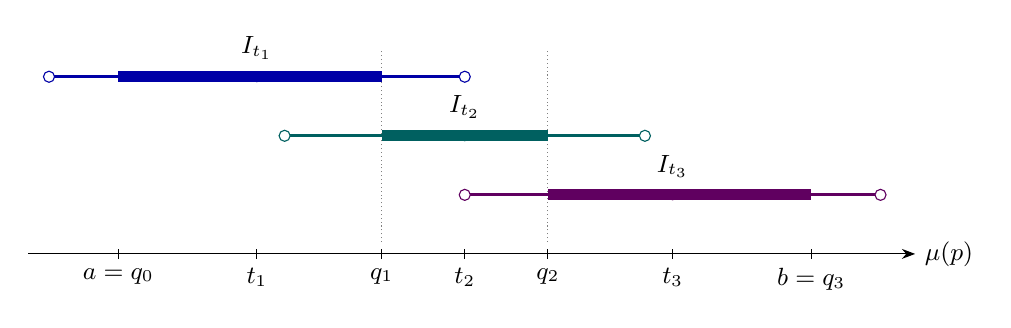
\begin{tikzpicture}[x=0.88cm,y=0.75cm,font=\small]
\draw[-{Stealth}] (-1.3,0)--(11.5,0) node[right] {$\mu(p)$};
\draw[densely dotted,gray] (3.8,0.2)--(3.8,3.45);
\draw[densely dotted,gray] (6.2,0.2)--(6.2,3.45);
\draw[blue!65!black,line width=1pt] (-1,3)--(5,3);
\draw[blue!65!black,line width=4pt] (0,3)--(3.8,3);
\draw[teal!75!black,line width=1pt] (2.4,2)--(7.6,2);
\draw[teal!75!black,line width=4pt] (3.8,2)--(6.2,2);
\draw[violet!75!black,line width=1pt] (5,1)--(11,1);
\draw[violet!75!black,line width=4pt] (6.2,1)--(10,1);
\draw[blue!65!black,fill=white] (-1,3) circle (2pt);
\draw[blue!65!black,fill=white] (5,3) circle (2pt);
\draw[teal!75!black,fill=white] (2.4,2) circle (2pt);
\draw[teal!75!black,fill=white] (7.6,2) circle (2pt);
\draw[violet!75!black,fill=white] (5,1) circle (2pt);
\draw[violet!75!black,fill=white] (11,1) circle (2pt);
\fill[blue!65!black] (2,3) circle (2pt);
\fill[teal!75!black] (5,2) circle (2pt);
\fill[violet!75!black] (8,1) circle (2pt);
\node[above] at (2,3.12) {$I_{t_1}$};
\node[above] at (5,2.12) {$I_{t_2}$};
\node[above] at (8,1.12) {$I_{t_3}$};
\draw (0,0.08)--(0,-0.08) node[below] {$a=q_0$};
\draw (2,0.08)--(2,-0.08) node[below] {$t_1$};
\draw (3.8,0.08)--(3.8,-0.08) node[below] {$q_1$};
\draw (5,0.08)--(5,-0.08) node[below] {$t_2$};
\draw (6.2,0.08)--(6.2,-0.08) node[below] {$q_2$};
\draw (8,0.08)--(8,-0.08) node[below] {$t_3$};
\draw (10,0.08)--(10,-0.08) node[below] {$b=q_3$};
\end{tikzpicture}
\caption{Finite gluing, schematically with three selected families.
The open intervals $I_{t_j}$ are the neighborhoods where the local
families approximate correctly. Each thick closed segment
$[q_{j-1},q_j]$ lies strictly inside its corresponding open interval.
For a label from family $j$ that stays active along a convergent sequence,
the common shifts in \eqref{eq:affine-shifts} force the limiting exponent
minimum $\mu(p)$ into that closed segment. Either adjacent family remains
valid when $\mu(p)$ equals a cut.}
\label{fig:interval-gluing}
\end{figure}


Suppose a fixed label from level $t_j$ is active in this combined family
along $h_\nu\to0+$ and $p^\nu\to p\in[a,b]^m$.  Write $c(h)$ for
its original local offset and again abbreviate $h=h_\nu$.  We claim
\[
  q_{j-1}\leq\mu(p)\leq q_j.
\]
If $j<N$ and $\mu(p)>q_j$, every $h^{p_i^\nu}$ is $o(h^{q_j})$.
The local offset is also $o(h^{q_j})$, by
Equation~\eqref{eq:affine-local-decay} and $q_j\in I_{t_j}$.
Subtracting the value of the label
$(t_{j+1}\mathbf 1,0)$ with its shift, the value difference is
\[
  (r-t_{j+1}\mathbf 1)\cdot X_h(p^\nu)+c(h)+h^{q_j}
  =h^{q_j}+o(h^{q_j})>0
\]
for all sufficiently large $\nu$, contradicting activity.

If $j>1$ and $\mu(p)<q_{j-1}$, subtract instead the shifted
label $(t_{j-1}\mathbf 1,0)$.  The difference is
\[
  (r-t_{j-1}\mathbf 1)\cdot X_h(p^\nu)+c(h)-h^{q_{j-1}}.
\]
Every coefficient in the scalar product is at least
$t_j-t_{j-1}>0$.  For some coordinate $i$, $p_i<q_{j-1}$, so
$h^{p_i^\nu}/h^{q_{j-1}}\to\infty$.  On the other hand,
$c(h)=o(h^{q_{j-1}})$ because $q_{j-1}<t_j<t_j+\rho_{t_j}$.
The displayed difference divided by $h^{q_{j-1}}$ therefore tends to
$+\infty$, again contradicting activity.  The outer bounds when $j=1$
or $j=N$ follow from $\mu(p)\in[a,b]$.

By Equation~\eqref{eq:affine-cuts}, the claimed bounds imply
$\mu(p)\in I_{t_j}$, including equality at either cut.  A label active
in the combined family is active within its original local family,
since all labels at that level received the same shift.  The guarantee
for $I_{t_j}$ now gives $\norm{p-r}_\infty<E(r)$.
All contradictions above produced a strictly smaller competing value,
so the argument applies to every active label even at ties.  This
completes the induction.
\end{proof}

The sequential conclusion gives a uniform estimate on the entire cube,
with the same fixed finite family. This is the form used for reaction
networks.

\begin{corollary}[Uniform activity bound]\label{cor:uniform-affine}
Let $m\ge1$, $a<b$, and $E:[a,b]^m\to(0,\infty)$ be as in
Lemma~\ref{lem:affine}. Fix a finite nonempty family
$\{(r_\lambda,c_\lambda):\lambda\in\Lambda\}$ supplied by that Lemma.
There is $h_0>0$ such that, for every $0<h<h_0$ and every
$p\in[a,b]^m$, each label active at $X_h(p)$ satisfies
\[
 \norm{p-r_\lambda}_\infty<E(r_\lambda).
\]
The family is fixed before $h_0$ is chosen.
\end{corollary}

\begin{proof}
Otherwise there are $h_\nu\to0+$, points $p^\nu\in[a,b]^m$, and
labels $\lambda_\nu$ active at $X_{h_\nu}(p^\nu)$ for which
\[
 \norm{p^\nu-r_{\lambda_\nu}}_\infty
 \ge E(r_{\lambda_\nu}).
\]
By finiteness of $\Lambda$ and compactness of $[a,b]^m$, a subsequence
has a fixed label $\lambda_\nu=\lambda$ and $p^\nu\to p\in[a,b]^m$.
Passing to the limit in the displayed inequality contradicts the strict
inequality in Lemma~\ref{lem:affine}. The value $E(r_\lambda)$ is fixed
on this subsequence, so no regularity of $E$ is used.
\end{proof}

In Section~\ref{sec:dynamics}, we choose the tolerance so that every
nonzero dot product of an active slope with a prescribed vector forces
the exponent vector to have a dot product of the same sign. The freedom
to choose a discontinuous $E$ permits this requirement near the corresponding
hyperplanes.

\section{From affine labels to persistent trajectories}
\label{sec:dynamics}

We now apply Lemma~\ref{lem:affine} to the mass-action vector field.
Its uniform form in Corollary~\ref{cor:uniform-affine} lets us choose
the tolerance so that every strict ordering made by an active slope gives
a monomial comparison with a definite gap. Weak reversibility converts those comparisons into
nonnegative derivatives, and an initially active constant branch supplies
the compact set that traps the trajectory.

\subsection{Uniform approximation and sign constraints}

Fix henceforth a network, positive rate constants, and
$x^0\in\R_{>0}^d$ as in Theorem~\ref{thm:main}. Write $e_1,\ldots,e_d$
for the standard basis of $\R^d$, and set
\begin{equation}\label{eq:comparison-directions}
 D=\{e_1,\ldots,e_d\}
 \cup\{z-y:y,z\in\mathcal C,\ y\ne z\}.
\end{equation}
Every vector in $D$ is nonzero. We include differences of \emph{all}
pairs of complexes, not only reaction vectors. The flux comparison below
compares the source of one upward reaction with the sources of every
downward reaction. Such sources need not be adjacent in the reaction
graph and may even belong to different linkage classes.

For $r\in[-1,1]^d$, define
\begin{equation}\label{eq:chosen-tolerance}
 E(r)=\min\left(
 \left\{\frac12\right\}
 \cup
 \left\{
 \frac{\abs{r\cdot v}}{2\norm{v}_1}:
 v\in D,\ r\cdot v\ne0
 \right\}\right),
 \qquad \norm{v}_1=\sum_{i=1}^d\abs{v_i}.
\end{equation}
This is a positive number for every $r$, since the displayed minimum is
over a finite nonempty set of positive numbers; in particular,
$E(0)=1/2$. The definition is allowed to be discontinuous at the
hyperplanes $r\cdot v=0$. This is the reason for allowing arbitrary
positive tolerances in Lemma~\ref{lem:affine}.

Apply that Lemma with $m=d$, $a=-1$, $b=1$, and the tolerance
\eqref{eq:chosen-tolerance}. Denote its fixed family by
$\{(r_\lambda,c_\lambda):\lambda\in\Lambda\}$ and put
\[
 F_h(x)=\min_{\lambda\in\Lambda}
       \bigl(r_\lambda\cdot x+c_\lambda(h)\bigr)
 \qquad(x\in\R^d).
\]
Choose $h_0\in(0,1)$ small enough that all offsets are defined and
Corollary~\ref{cor:uniform-affine} applies for $0<h<h_0$.
Before choosing a particular $h$, define
\begin{equation}\label{eq:fixed-gap}
 H=\min\left(
 \{1\}\cup
 \left\{
 \frac12\abs{r_\lambda\cdot v}:
 \lambda\in\Lambda,\ v\in D,\ r_\lambda\cdot v\ne0
 \right\}\right)>0.
\end{equation}
The positivity of $H$ again follows from finiteness. Both the slopes and
$H$ are independent of the eventual choice of $h$.
Thus the order of choices is
\[
 D\ \longrightarrow\ E\ \longrightarrow\ \Lambda
 \ \longrightarrow\ (h_0,H)\ \longrightarrow\ h.
\]
In particular, $H$ is not a separation parameter that is allowed to tend
to zero together with $h$.

Suppose that $0<h<h_0$, $p\in[-1,1]^d$, and $\lambda$ is active at
$X_h(p)$. For every $v\in D$ with $r_\lambda\cdot v\ne0$, we have
\begin{align*}
 \abs{(p-r_\lambda)\cdot v}
 &\le \norm{p-r_\lambda}_\infty\norm{v}_1\\
 &<E(r_\lambda)\norm{v}_1
 \le\frac12\abs{r_\lambda\cdot v}.
\end{align*}
Consequently,
\begin{equation}\label{eq:sign-and-gap}
 \operatorname{sgn}(p\cdot v)
 =\operatorname{sgn}(r_\lambda\cdot v),
 \qquad \abs{p\cdot v}\ge H.
\end{equation}
In particular, $\abs{p\cdot v}<H$ forces $r_\lambda\cdot v=0$.
Thus a comparison too close to a tie in exponent space is made an exact
tie by the active slope. The converse is not required: equal slope levels
may contain complexes with different monomial values.
For $x=X_h(p)$ and any $y,z\in\mathcal C$, this implies
\begin{equation}\label{eq:monomial-order}
 r_\lambda\cdot y<r_\lambda\cdot z
 \quad\Longrightarrow\quad
 x^z\le h^H x^y.
\end{equation}
Indeed, $z-y\in D$ and $p\cdot(z-y)\ge H$, while
$x^z/x^y=h^{p\cdot(z-y)}$ and $0<h<1$.

We can now fix a single $h\in(0,h_0)$ satisfying
\begin{equation}\label{eq:initial-exponents}
 p_i^0=\frac{\log x_i^0}{\log h},
 \qquad \norm{p^0}_\infty<H,
\end{equation}
and, when $\mathcal R\ne\varnothing$, also satisfying
\begin{equation}\label{eq:rate-separation}
 h^H\sum_{e\in\mathcal R}\kappa_e
 <\min_{e\in\mathcal R}\kappa_e.
\end{equation}
This choice is possible because $p^0\to0$ and $h^H\to0$ as
$h\to0+$, with $H>0$ already fixed. No minimum of reaction rates is
needed when $\mathcal R$ is empty. Write
\[
 B_h=[h,h^{-1}]^d,
 \qquad F=F_h.
\]
Since $H\le1$, Equation~\eqref{eq:initial-exponents} places $x^0$ in
the interior of $B_h$.

Every label active at $x^0$ has slope zero. In fact, if its $i$th slope
coordinate were nonzero, Equation~\eqref{eq:sign-and-gap} applied to
$v=e_i$ would give $\abs{p_i^0}\ge H$, contradicting
\eqref{eq:initial-exponents}. The finite nonempty family has at least
one active label; fix such a label $\lambda_0$ and put $M=F(x^0)$. Then
\begin{equation}\label{eq:ceiling}
 r_{\lambda_0}=0,
 \qquad M=F(x^0)=c_{\lambda_0}(h),
 \qquad F(x)\le M\quad(x\in\R^d).
\end{equation}
Thus a constant branch is forced by the sign constraints, even though it
was not prescribed in the application of Lemma~\ref{lem:affine}.

There is no point $x\in\partial B_h$ at which $F(x)=M$. To see this,
write $x=X_h(p)$ with $p\in[-1,1]^d$. The boundary condition is
$\norm{p}_\infty=1$. Equality $F(x)=M$ would make $\lambda_0$ active,
so Corollary~\ref{cor:uniform-affine} would instead give
$\norm{p}_\infty<E(0)=1/2$. We have proved
\begin{equation}\label{eq:no-boundary-plateau}
 \{x\in B_h:F(x)=M\}\cap\partial B_h=\varnothing.
\end{equation}
Thus the maximum set $\{F=M\}$ contains $x^0$ and misses
$\partial B_h$. To prove its invariance, we next show that a trajectory
segment in $B_h$ cannot decrease $F$. The constant branch alone does not prove this: another branch tied
with it might otherwise become smaller. We must control the derivatives
of all active branches. The next two arguments establish that control
from weak reversibility.

\subsection{Flux across the ordered complex levels}

The following finite graph statement isolates the role of weak
reversibility. Its weights will be the monomials $x^y$, and its levels
will be the scalar products $r_\lambda\cdot y$.

\begin{lemma}[Flux across level cuts]\label{lem:cut-flux}
Let $V$ be a finite set and $\mathcal E$ a finite set of directed edges
with source and target maps $s,t:\mathcal E\to V$. Suppose that for
every edge there is a directed path from its target back to its source.
Let $a:V\to\R$, let $w_v>0$ for $v\in V$, and let
$\kappa_e>0$ for $e\in\mathcal E$. Assume that there is $\delta>0$
such that
\begin{equation}\label{eq:abstract-weight-order}
 a(u)<a(z)\quad\Longrightarrow\quad w_z\le\delta w_u
 \qquad(u,z\in V).
\end{equation}
If $\mathcal E\ne\varnothing$, assume in addition that
\[
 \delta\sum_{e\in\mathcal E}\kappa_e
 <\min_{e\in\mathcal E}\kappa_e.
\]
Then
\[
 \sum_{e\in\mathcal E}
 \kappa_e w_{s(e)}\bigl(a(t(e))-a(s(e))\bigr)\ge0.
\]
\end{lemma}

\begin{proof}
The sum is zero if $\mathcal E$ is empty, including the case of an empty
vertex set. Otherwise list the distinct values of $a$ as
$\alpha_1<\cdots<\alpha_q$. For $1\le j<q$, let
\[
 V_j^- =\{v\in V:a(v)\le\alpha_j\},
 \qquad V_j^+=V\setminus V_j^-.
\]
Let $\mathcal E_j^+$ consist of edges from $V_j^-$ to $V_j^+$ and
$\mathcal E_j^-$ of edges in the reverse direction. Define their net
upward flux by
\[
 Q_j=\sum_{e\in\mathcal E_j^+}\kappa_e w_{s(e)}
      -\sum_{e\in\mathcal E_j^-}\kappa_e w_{s(e)}.
\]
If $\mathcal E_j^-\ne\varnothing$, take one of its edges. Its return
path starts in $V_j^-$ and ends in $V_j^+$, so that path contains an edge
$e_0\in\mathcal E_j^+$. Put $u=s(e_0)$. Every source $z$ of an edge
in $\mathcal E_j^-$ satisfies $a(z)>a(u)$, and hence
\begin{align*}
 \sum_{e\in\mathcal E_j^-}\kappa_e w_{s(e)}
 &\le \delta w_u\sum_{e\in\mathcal E_j^-}\kappa_e\\
 &\le \delta w_u\sum_{e\in\mathcal E}\kappa_e
 <w_u\min_{e\in\mathcal E}\kappa_e
 \le \kappa_{e_0}w_u.
\end{align*}
It follows that $Q_j>0$. If $\mathcal E_j^-$ is empty, then $Q_j\ge0$
directly.
Notice that the selected edge $e_0$ need not share a component with every
downward edge. The all-pairs hypothesis
\eqref{eq:abstract-weight-order} is what permits one upward contribution
to dominate the entire downward sum in this proof.

For each edge, its level difference is the signed sum of the gaps
$\alpha_{j+1}-\alpha_j$ over the cuts it crosses. Summing this identity
over the finite edge set gives
\begin{equation}\label{eq:cut-decomposition}
 \sum_{e\in\mathcal E}
 \kappa_e w_{s(e)}\bigl(a(t(e))-a(s(e))\bigr)
 =\sum_{j=1}^{q-1}(\alpha_{j+1}-\alpha_j)Q_j\ge0.
\end{equation}
When $q=1$, both sides vanish. Equal vertex levels therefore cause no
difficulty, and no connectedness assumption has entered the argument.
\end{proof}

Return-path monomial domination appears in Anderson's tier
argument~\cite[Lemma~4.7]{Anderson2011Global}, and quantitative inward
reaction estimates underlie the invariant polygons of Craciun, Nazarov,
and Pantea~\cite{CraciunNazarovPantea2013}. Ordered-cut regrouping also
appears in the proof of Craciun's toric-inclusion embedding
theorem~\cite[preprint, Theorem~4.1]{Craciun2019}. Lemma~\ref{lem:cut-flux}
uses a direct finite estimate: one upward edge dominates the full downward
flux. No tier extraction, cycle decomposition, or differential inclusion
is required in the proof above.

For any $x\in B_h$ and any label $\lambda$ active at $x$, apply
Lemma~\ref{lem:cut-flux} with
\[
 V=\mathcal C,\quad \mathcal E=\mathcal R,\quad
 a(y)=r_\lambda\cdot y,\quad w_y=x^y,\quad \delta=h^H.
\]
The return paths are supplied by weak reversibility,
Equation~\eqref{eq:monomial-order} supplies
\eqref{eq:abstract-weight-order}, and
Equation~\eqref{eq:rate-separation} supplies the rate inequality when
there are reactions. Thus
\begin{equation}\label{eq:active-nondecrease}
 r_\lambda\cdot f(x)
 =\sum_{y\to y'\in\mathcal R}
   \kappa_{y\to y'}x^y\,r_\lambda\cdot(y'-y)
 \ge0
 \qquad(x\in B_h,\ \lambda\text{ active at }x).
\end{equation}
This includes $f=0$ for an empty reaction set. The comparison in
\eqref{eq:abstract-weight-order} is required for all ordered vertex
pairs, including nonadjacent pairs in one component and pairs in different
components; this explains the full set of complex differences in
\eqref{eq:comparison-directions}.

\subsection{Derivatives of finite affine minima}

Although $F$ need not be differentiable where its active labels change,
its right derivative along a differentiable curve is explicit. We record
the finite-affine minimum case of the classical active-branch
directional-derivative principle; see, for example,
Bertsekas~\cite[Proposition~A.3.2(a)]{Bertsekas2009} for the corresponding
maximum formula. The short proof includes all ties and the monotonicity
implication needed here.

\begin{lemma}[Right derivative of a finite affine minimum]
\label{lem:minimum-derivative}
Let $I$ be a finite nonempty index set, let $b_i\in\R^d$ and
$d_i\in\R$ for $i\in I$, and define
\[
 \Phi(x)=\min_{i\in I}(b_i\cdot x+d_i),
 \qquad A(x)=\{i\in I:b_i\cdot x+d_i=\Phi(x)\}.
\]
For a continuously differentiable curve
$\gamma:[u,v]\to\R^d$, the right derivative at every $\tau\in[u,v)$
exists and is
\[
 \frac{d^+}{d\tau}\Phi(\gamma(\tau))
 =\min_{i\in A(\gamma(\tau))} b_i\cdot\gamma'(\tau).
\]
If $b_i\cdot\gamma'(\tau)\ge0$ for every $\tau\in[u,v)$ and every
$i\in A(\gamma(\tau))$, then $\Phi\circ\gamma$ is nondecreasing on
$[u,v]$.
\end{lemma}

\begin{proof}
Fix $\tau<v$. Each inactive branch has a strictly positive gap above
any chosen active branch at $\gamma(\tau)$. By continuity and finiteness,
every inactive branch stays above that chosen branch at
$\gamma(\tau+\eta)$ for sufficiently small $\eta\ge0$. For the remaining
branches, the first-order expansions, uniform over the finite active set,
give
\[
 \Phi(\gamma(\tau+\eta))
 =\Phi(\gamma(\tau))
  +\eta\min_{i\in A(\gamma(\tau))}
       b_i\cdot\gamma'(\tau)+o(\eta)
 \qquad(\eta\downarrow0).
\]
This proves the right derivative formula, including at ties.

Under the stated nonnegativity hypothesis, take any
$u\le s<t\le v$ and any $\epsilon>0$. The continuous function
\[
 g(\tau)=\Phi(\gamma(\tau))+\epsilon\tau
 \qquad(s\le\tau\le t)
\]
has strictly positive right derivative at every $\tau<t$. It cannot
attain its maximum at such a point, because sufficiently small positive
increments would increase its value. Compactness therefore places its
maximum at $t$, giving $g(s)\le g(t)$. Letting $\epsilon\downarrow0$
proves $\Phi(\gamma(s))\le\Phi(\gamma(t))$.
\end{proof}

\subsection{The invariant polytope and trajectory bounds}

All active branches have nonnegative derivative in $B_h$, while the
constant branch in \eqref{eq:ceiling} gives $F\le M$ everywhere. We now
show that the maximum set of $F$ is the compact invariant polytope
announced in the introduction. Its invariance will give
Theorem~\ref{thm:main}.

Nonnegative derivatives on all active inequalities express the familiar
inward-tangency condition for invariance, whose classical general form
goes back to Nagumo~\cite{Nagumo1942}. Here we prove invariance directly
by a first-exit argument.

\begin{proposition}\label{prop:polytope}
For every finite weakly reversible mass-action network with positive
constant rates, and every $x^0\in\R_{>0}^d$, there is a compact convex
polytope $K\subset\R_{>0}^d$ containing $x^0$ and forward invariant for
the mass-action equation. Here forward invariance means that every
solution starting in $K$ exists for all forward time and stays in $K$.
\end{proposition}

\begin{proof}
Use the family, $h$, $F$, $M$, and $B_h$ constructed above, and set
\begin{equation}\label{eq:polytope}
 K=\{x\in\R^d:F(x)=M\}
  =\bigcap_{\lambda\in\Lambda}
    \{x\in\R^d:r_\lambda\cdot x+c_\lambda(h)\ge M\}.
\end{equation}
The equality follows from $F\le M$. Thus $K$ is a closed convex
polyhedron containing $x^0$, and \eqref{eq:no-boundary-plateau} gives
$K\cap\partial B_h=\varnothing$.

In fact $K\subset\operatorname{int}B_h$. Otherwise a segment from
$x^0\in\operatorname{int}B_h$ to a point of $K$ outside that interior
would lie in $K$ by convexity and meet $\partial B_h$, a contradiction.
Therefore $K$ is bounded as well as closed, so it is a compact convex
polytope in $\R_{>0}^d$. This step uses no active-label estimate outside
the box.

Let $z\in K$. Since the polynomial vector field $f$ is smooth on
$\R^d$, it has a unique local solution $x$ from $z$ with a maximal
forward existence interval $[0,T_{\max})$. We initially regard this as
a solution in $\R^d$; confinement below will give positivity.
On any interval $[0,T]\subset[0,T_{\max})$ for which
$x([0,T])\subset B_h$, \eqref{eq:active-nondecrease} and
Lemma~\ref{lem:minimum-derivative} make $F(x(t))$ nondecreasing.
Since $F(z)=M$ and $F\le M$, we obtain
\begin{equation}\label{eq:trajectory-plateau}
 F(x(t))=M\qquad(0\le t\le T).
\end{equation}

The point $z$ lies in the interior of $B_h$. If the solution reached
the boundary at a first time $\tau<T_{\max}$, its whole segment
$x([0,\tau])$ would lie in $B_h$. Applying
\eqref{eq:trajectory-plateau} to that closed segment would give
$F(x(\tau))=M$, contrary to \eqref{eq:no-boundary-plateau}.
Continuity shows that any departure from the interior before
$T_{\max}$ would have such a first boundary time. Hence
$x(t)\in\operatorname{int}B_h$ for all $0\le t<T_{\max}$, and
\eqref{eq:trajectory-plateau} places the whole trajectory in $K$.

If $T_{\max}<\infty$, continuity of $f$ on the compact box gives
$L<\infty$ with $\norm{f(x)}\le L$ for $x\in B_h$. Consequently
\[
 \norm{x(t)-x(s)}\le L\abs{t-s}
 \qquad(0\le s,t<T_{\max}),
\]
so $x(t)$ has a limit $\bar x\in K\subset B_h$ as
$t\uparrow T_{\max}$. Local existence from $\bar x$ extends the
solution past $T_{\max}$: the original integral equation passes to
the endpoint, and both one-sided derivatives there equal $f(\bar x)$.
This contradicts maximality. Thus $T_{\max}=\infty$, proving the
claimed forward invariance for every $z\in K$.
\end{proof}

\begin{proof}[Proof of Theorem~\ref{thm:main}]
For the prescribed $x^0$, Proposition~\ref{prop:polytope} and its
construction give a forward-invariant polytope
$x^0\in K\subset B_h=[h,h^{-1}]^d$ with $0<h<1$. The solution
therefore exists globally and satisfies
\[
 h\le x_i(t)\le h^{-1}\qquad(t\ge0,\ 1\le i\le d).
\]
Taking $\varepsilon=h$ gives \eqref{eq:main-bounds}. Each coordinate
has positive infimum on the entire forward trajectory, and hence
positive forward limit inferior.
\end{proof}

\subsection{Equilibria and complex-balanced convergence}

The convexity of the invariant set also recovers the known existence of
positive equilibria in every positive stoichiometric class, proved by
Boros~\cite[preprint, Theorem~1]{Boros2019}.

\begin{corollary}\label{cor:positive-equilibrium}
For every finite weakly reversible mass-action network with positive
constant rates and every $x^0\in\R_{>0}^d$, there is an equilibrium
$x^*\in(x^0+S)\cap\R_{>0}^d$.
\end{corollary}

\begin{proof}
Let $K$ be the polytope in Proposition~\ref{prop:polytope}. The set
$Q=K\cap(x^0+S)$ is nonempty, compact, convex, and forward invariant.
Write $\phi_t$ for the flow. For each integer $n\ge1$, the continuous
map $\phi_{1/n}:Q\to Q$ has a fixed point $z_n$ by Brouwer's theorem.
Thus
\[
 0=n\bigl(\phi_{1/n}(z_n)-z_n\bigr)
   =n\int_0^{1/n}f(\phi_s(z_n))\,ds.
\]
Put $L=\max_{z\in Q}\norm{f(z)}$. Invariance and the integral equation
give $\norm{\phi_s(z_n)-z_n}\le L/n$ for $0\le s\le1/n$.
Uniform continuity of $f$ on $Q$ therefore yields
\[
 \norm{f(z_n)}
 \le\sup_{0\le s\le1/n}\norm{f(\phi_s(z_n))-f(z_n)}
 \longrightarrow0.
\]
A subsequence of $z_n$ converges to some $x^*\in Q$, and continuity gives
$f(x^*)=0$. Since $Q\subset\R_{>0}^d$, this is the required positive
equilibrium.
\end{proof}

\begin{remark}[Complex-balanced convergence]
\label{rem:complex-balanced-convergence}
Under the additional assumption of complex balance,
Theorem~\ref{thm:main} recovers the known global-attractor conclusion
(see also \cite{Craciun2026}): for fixed positive rate constants, every
positive trajectory converges to the unique positive equilibrium in its
positive stoichiometric class $P\cap\R_{>0}^d$.
Indeed, complex balance implies weak reversibility, and
Proposition~\ref{prop:polytope} traps the trajectory in the compact positive
forward-invariant set $K\cap(x^0+S)$. Let $x^*$ be the unique positive
equilibrium in this class. The Horn--Jackson entropy function
\[
 V(x)=\sum_{i=1}^d
 \left(x_i\log\frac{x_i}{x_i^*}-x_i+x_i^*\right)
\]
is nonincreasing and has zero derivative only at equilibria. This
dissipation property and uniqueness in each positive class are the
standard complex-balance conclusions
\cite[Proposition~5.3 and Corollaries~5.4--5.5]{FeinbergLectures1979}.
LaSalle's invariance principle therefore gives convergence.
In particular, the conclusion holds for every fixed positive rate choice
on every weakly reversible deficiency-zero network
\cite[Corollary~5.10]{FeinbergLectures1979}. Here the deficiency is
$|\mathcal C|-\ell-\dim S$, where $\ell$ is the number of linkage classes.
\end{remark}

\bibliographystyle{plainnat}
\bibliography{references}
\end{document}
